\section{Set Theory and Logic}

\begin{exercise} \label{0.1}
	pending
\end{exercise}

\begin{exercise} \label{0.2}
	pending
\end{exercise}

\begin{exercise} \label{0.3}
	pending
\end{exercise}

\begin{exercise} \label{0.4}
	pending
\end{exercise}

\begin{exercise} \label{0.5}
	pending
\end{exercise}

\begin{exercise} \label{0.6}
	pending
\end{exercise}

\begin{exercise} \label{0.7}
	pending
\end{exercise}

\begin{exercise} \label{0.8}
	pending
\end{exercise}

\begin{exercise} \label{0.9}
	pending
\end{exercise}

\begin{exercise} \label{0.10}
	pending
\end{exercise}

\begin{exercise} \label{0.11}
	pending
\end{exercise}

\begin{exercise} \label{0.12}
	Two sets $A$ and $B$ are such that their union and their intersection are equal. What can we say about $A$ and $B$?
	
	\begin{proof}
	    We see that
	    $$ B \subseteq A \cup B = A \cap B \subseteq A $$
	    and
	    $$ A \subseteq A \cup B = A \cap B \subseteq B $$
	    which implies that $A=B$.
	\end{proof}
\end{exercise}

\begin{exercise} \label{0.13}
	Suppose that $A$ is a subset of $B$ and $C$ is a subset of $D$.
	
	\begin{enumerate}[label=(\alph*)]
	    \item Is it true that $A \cup C$ is a subset of $B \cup D$?
	    \item Is it true that the intersection of $A$ and $C$ is a subset of the intersection of $B$ and $D$?
	\end{enumerate}
	
	\begin{proof}
	    \begin{enumerate}[label=(\alph*)]
	        \item Notice
	        $$ A \subseteq B \cup D $$
	        and
	        $$ C \subseteq B \cup D $$
	        thus
	        $$ (A \cup C) \subseteq (B \cup D) $$
	        
	        \item Let $x \in A \cap C$. So $x \in A$ and $x \in C$. So $x \in B$ and $x \in D$. So $x \in B \cap D$. Therefore $A \cap C \subseteq B \cap D$.
	    \end{enumerate}
	\end{proof}
\end{exercise}

\begin{exercise} \label{0.14}
	what can we say about two sets $P$ and $Q$ if $P - Q$ is equal to $Q - P$?
	
	\begin{proof}
	    Note that
	    $$ x \in P-Q \Rightarrow  x \not\in Q \Rightarrow x \not\in Q-P $$
	    Thus, the assumption of equality implies that $P-Q=Q-P=\emptyset$. This, in turn, implies $P=Q$.
	\end{proof}
\end{exercise}

\begin{exercise} \label{0.15}
	Let $A$ and $B$ be non-empty sets. Prove that if $A \times B = B \times A$ then $A=B$.
	
	\begin{proof}
	    Let $(a,b) \in A \times B$. By $A \times B = B \times A$, there exists $(b',a') \in B \times A$ such that $a=b'$ and $b=a'$. Thus $A \subseteq B$ and $B \subseteq A$. Therefore $A=B$.
	\end{proof}
\end{exercise}

\begin{exercise} \label{0.16}
	What is the cardinality of $P \times Q$ if the cardinality of $P$ is $p$ and the cardinality of $Q$ is $q$?
	
	\begin{proof}
	    We can denote
	    $$ P = \{ x_1, x_2, \ldots, x_p \} $$
	    $$ Q = \{ y_1, y_2, \ldots, y_q \} $$
	    Thus
	    \begin{align*}
	        P \times Q &= \{ (x_1,y_i): 1 \leq i \leq q \} \cup \{ (x_2,y_i): 1 \leq i \leq q \} \cup \ldots \cup \{ (x_p,y_i): 1 \leq i \leq q \} \\
	        &= S_1 \cup S_2 \cup \ldots \cup S_p
	    \end{align*}
	    where $S_i \cap S_j = \emptyset$ whenever $i \neq j$ and $\vert S_i \vert = q$ for $1 \leq i \leq p$. Thus 
	    \begin{align*}
	        \vert P \times Q \vert &= \sum_{i=1}^{p} \vert S_i \vert \\
	        &= \sum_{i=1}^{p} q \\
	        &= pq
	    \end{align*}
	\end{proof}
\end{exercise}

\begin{exercise} \label{0.17}
	Prove that the intersection of the powerset of $A$ and the powerset of $B$ is the powerset of the intersection of $A$ and $B$, where $A$ and $B$ are two arbitrary sets.
	
	\begin{proof}
	    \begin{align*}
	        x \in 2^{A} \cap 2^{B} &\iff x \subseteq A \text{ and } x \subseteq B \\
	        &\iff x \subseteq A \cap B \\
	        &\iff x \in 2^{A \cap B}
	    \end{align*}    
	\end{proof}
\end{exercise}

\begin{exercise} \label{0.18}
	pending
\end{exercise}

\begin{exercise} \label{0.19}
	What is the cardinality of the powerset of the empty set?
	
	\begin{proof}
	    $2^\emptyset = \{ \emptyset \}$. Thus $\left| 2^\emptyset \right| = 1$.
	\end{proof}
\end{exercise}

\begin{exercise} \label{0.20}
	If the power set of $A$ is equal to the powerset of $B$ does it follow that $A$ and $B$ are equal?
	
	\begin{proof}
	    Yes it does for, suppose to the contrary, that $x \in A - B$. Then $\{ x \} \in 2^A$ and $\{x\}\not\in 2^B$ contradicting with $2^A=2^B$. The same reasoning applies for $x \in B - A$. Thus $A=B$.
	\end{proof}
\end{exercise}

\begin{exercise} \label{0.21}
	pending
\end{exercise}

\begin{exercise} \label{0.22}
	pending
\end{exercise}

\begin{exercise} \label{0.23}
	pending
\end{exercise}

\begin{exercise} \label{0.24}
	pending
\end{exercise}

\begin{exercise} \label{0.25}
	pending
\end{exercise}

\begin{exercise} \label{0.26}
	pending
\end{exercise}

\begin{exercise} \label{0.27}
	pending
\end{exercise}

\begin{exercise} \label{0.28}
	pending
\end{exercise}

\begin{exercise} \label{0.29}
	pending
\end{exercise}

\begin{exercise} \label{0.30}
	pending
\end{exercise}

\begin{exercise} \label{0.31}
	pending
\end{exercise}

\begin{exercise} \label{0.32}
	pending
\end{exercise}

\begin{exercise} \label{0.33}
	pending
\end{exercise}

\begin{exercise} \label{0.34}
	pending
\end{exercise}

\begin{exercise} \label{0.35}
	Find the domain and range of the function that assigns 
	\begin{enumerate}[label=(\alph*)]
	    \item each integer its last digit
	    \item each integer the number of digits in it.
	\end{enumerate}
	    
	\begin{proof}
	    \begin{enumerate}[label=(\alph*)]
	        \item Domain: $\mathbb{Z}$
	        Range: $\{ 0,1,2,\ldots,9 \}$
	        
	        \item Domain: $\mathbb{Z}$
	        Range: $\mathbb{N}$
	    \end{enumerate}
	\end{proof}
\end{exercise}

\begin{exercise} \label{0.36}
	pending
\end{exercise}

\begin{exercise} \label{0.37}
	pending
\end{exercise}

\begin{exercise} \label{0.38}
	pending
\end{exercise}

\begin{exercise} \label{0.39}
	pending
\end{exercise}

\begin{exercise} \label{0.40}
	Show that the set of all positive integers is equivalent to the set of all positive even integers
	
	\begin{proof}
	    Take $f(n)=2n$. Then $f$ is a bijection between the set of positive integers and the set of all positive even integers. To demonstrate surjectivity: $n \rightarrow 2n$ for $2n$ a positive even integer. To demonstrate injectivity: if $f(n)=f(n')$ then 
	    \begin{align*}
	        2n &= 2n' \\
	        n &= n'
	    \end{align*}
	\end{proof}
\end{exercise}

\begin{exercise} \label{0.41}
	pending
\end{exercise}

\begin{exercise} \label{0.42}
	pending
\end{exercise}

\begin{exercise} \label{0.43}
	pending
\end{exercise}

\begin{exercise} \label{0.44}
	Suppose that $f:X \rightarrow Y$ and $A$ and $B$ are subsets of $X$. Then prove:
	\begin{enumerate}[label=(\alph*)]
	    \item $f\left( A \cup B \right) = f(A) \cup f(B)$
	    \item`$f(A\cap B) \subseteq f(A) \cap f(B)$
	\end{enumerate}
	
	\begin{proof}
	    \begin{enumerate}[label=(\alph*)]
	        \item 
	        \begin{align*}
	            y \in f(A \cup B) &\Leftrightarrow \exists x \in A \cup B \text{ s.t. } y = f(x) \\
	            &\Leftrightarrow \exists a \in A \text{ s.t. } y=f(a) \\
	            &\text{ } \hspace{4mm} \text{ or } \exists b \in B \text{ s.t. } y = f(b) \\
	            &\Leftrightarrow y \in f(A) \cup f(B)
	        \end{align*}
	        \item
	        \begin{align*}
	            y \in f(A \cap B) &\Leftrightarrow \exists x \in A \cap B \text{ s.t. } y = f(x) \\
	            &\Rightarrow \exists a \in A \text{ s.t. } y=f(a) \\
	            &\text{ } \hspace{4mm} \text{ and } \exists b \in B \text{ s.t. } y = f(b) \\
	            &\Leftrightarrow y \in f(A) \cup f(B)
	        \end{align*}
	    \end{enumerate}
	\end{proof}
\end{exercise}

\begin{exercise} \label{0.45}
	Show that if $f:X \rightarrow Y$ is an injection, then $f(A \cap B)=f(A) \cap f(B)$ for all subsets $A$ and $B$ of $X$.
	
	\begin{proof}
	    Let $y=f(x)$
	    \begin{align*}
	        y \in f(A \cap B) &\Leftrightarrow x \in A \cap B \\
	        &\Leftrightarrow x \in A \text{ and } x \in B \\
	        &\Leftrightarrow  y \in f(A) \cap f(B)
	    \end{align*}
	\end{proof}
\end{exercise}

\begin{exercise} \label{0.46}
	Show that there is an injection from $A$ to $B$ if and only if there is a surjection from $B$ to $A$.
	
	\begin{proof}
	    
	\end{proof}
\end{exercise}

\begin{exercise} \label{0.47}
	Suppose that $f:A \rightarrow B$ where $A$ and $B$ are two finite sets with same cardinality. Prove that $f$ is an injection if and only if $f$ is a surjection. 
	
	\begin{proof}
	    hello
	\end{proof}
\end{exercise}

\begin{exercise} \label{0.48}
	pending
\end{exercise}

\begin{exercise} \label{0.49}
	pending
\end{exercise}

\begin{exercise} \label{0.50}
	pending
\end{exercise}

\begin{exercise} \label{0.51}
	pending
\end{exercise}

\begin{exercise} \label{0.52}
	pending
\end{exercise}

\begin{exercise} \label{0.53}
	pending
\end{exercise}

\begin{exercise} \label{0.54}
	pending
\end{exercise}

\begin{exercise} \label{0.55}
	pending
\end{exercise}

\begin{exercise} \label{0.56}
	pending
\end{exercise}

\begin{exercise} \label{0.57}
	pending
\end{exercise}

\begin{exercise} \label{0.58}
	pending
\end{exercise}

\begin{exercise} \label{0.59}
	pending
\end{exercise}

\begin{exercise} \label{0.60}
	pending
\end{exercise}

\begin{exercise} \label{0.61}
	pending
\end{exercise}

\begin{exercise} \label{0.62}
	pending
\end{exercise}

\begin{exercise} \label{0.63}
	pending
\end{exercise}

\begin{exercise} \label{0.64}
	pending
\end{exercise}

\begin{exercise} \label{0.65}
	Let \( R = \{ (x,y): x,y \in \mathbb{R} \text{ and } x-y \in \mathbb{Z} \} \). Show that \( R \) is an equivalence relation.
	
	\begin{proof}
	    Recall that a relation is an equivalence relation when it is reflexive, symmetric, and transitive. Thus we wish to show that \( R \) is reflexive, symmetric, and transitive.
	    
	    To show that \( R \) is reflexive \( x - x = 0 \in \mathbb{Z} \). To show that \( R \) is symmetric, we observe that if \( x - y \in \mathbb{Z} \) then \( y - x = -(x-y) \in \mathbb{Z} \) so that \( R \) is symmetric. Finally, to show that \( R \) is transitive, if \( x - y, y - z \in \mathbb{R} \) then 
	    \[ x - z = (x - y) + (y - z) \in \mathbb{Z} \]
	\end{proof}
\end{exercise}

\begin{exercise} \label{0.66}
	\begin{enumerate}
	    \item \( a (mod \hspace{1mm} m) = b (mod \hspace{1mm} m) \) if and only if \( a \equiv b (mod \hspace{1mm} m) \)
	    
	    \item \( a \equiv b (mod \hspace{1mm} m) \) if and only if there exists an integer \( k \) such that \( a = b + km \)
	    
	    \item If \( a \equiv b (mod \hspace{1mm} m) \) and \( c \equiv d (mod \hspace{1mm} m) \), then \( a + c \equiv (b+d) (mod \hspace{1mm} m) \) and \( ac \equiv bd (mod \hspace{1mm} m) \)
	\end{enumerate}
	    \begin{proof}
	        \begin{enumerate}
	            \item \( a \equiv b \hspace{1mm} (mod \hspace{1mm} m) \) iff
	            \begin{align*}
	                a-b = qm &\text{ iff } a = qm+b = km + a \hspace{1mm} (mod \hspace{1mm} m) \\
	                &\text{ iff } b-a \hspace{1mm}(mod \hspace{1mm} m) = km - qm \\
	                &\text{ iff } b-a \hspace{1mm}(mod \hspace{1mm} m)=(k-q)m \\
	                &\text{ iff } b=(k-q)m+a \hspace{1mm} (mod \hspace{1mm} m) \\
	                &\text{ iff } a \hspace{1mm} (mod \hspace{1mm} m) = b \hspace{1mm} (mod \hspace{1mm} m)
	            \end{align*}
	            
	            \item \( a - b = km \text{ iff } a = b + km \)
	            
	            \item We have \( a - b = qm \) and \( c - d = km \). Thus 
	            \[ (a+c) - (b+d) = (a-b) + (c-d) = qm + km = (q+k)m \]
	            Therefore, \( a+c \equiv b+d \hspace{1mm} (mod \hspace{1mm} m) \). 
	            
	            For multiplication
	            \begin{align*}
	                ac - bd &= ac - (a - qm)(c - km) \\
	                &= ac - (ac - akm - cqm + qkm^2) \\
	                &= ac - ac + akm + cqm - qkm^2 \\
	                &= akm + cqm - qkm^2 \\
	                &= (ak + cq - qkm)m
	            \end{align*}
	            implying \( ac \equiv bd \hspace{1mm} (mod \hspace{1mm} m) \)
	        \end{enumerate}
	    \end{proof}
\end{exercise}

\begin{exercise} \label{0.67}
	Show that congruence modulo m is an equivalence relation
	\begin{proof}
	    To show the relation is reflexive we observe \( a - a = 0m \) iff \( a \equiv a \hspace{1mm} (mod \hspace{1mm} m) \)
	    
	    To show that the relation is symmetric we let \( a \equiv b \hspace{1mm} (mod \hspace{1mm} m) \). So \( a - b = qm \). So \( b - a = -qm \). So \( b \equiv a \hspace{1mm} (mod \hspace{1mm} m) \).
	    
	    To show transitivity, let \( a \equiv b \hspace{1mm} (mod \hspace{1mm} m) \) and \( b \equiv c \hspace{1mm} (mod \hspace{1mm} m) \). So \( a - b = qm \) and \( b - c = km \). So
	    \[ a - c = a - b + b -c = (a - b) + (b - c) = qm + km = (q+k)m \]
	    Therefore \( a \equiv c \hspace{1mm} (mod \hspace{1mm} m) \).
	\end{proof}
\end{exercise}

\begin{exercise} \label{0.68}
	Find the congruence classes modulo 5:
	\begin{enumerate}
	    \item \( [0]_5 \)
	    \item \( [1]_5 \)
	    \item \( [2]_5 \)
	\end{enumerate}
	
	\begin{proof}
	    \begin{enumerate}
	        \item \( [0]_5 = \{ x : x = 5q + 0, q \in \mathbb{Z} \} \)
	        \item \( [1]_5 = \{ x : x = 5q + 1, q \in \mathbb{Z} \} \)
	        \item \( [2]_5 = \{ x : x = 5q + 2, q \in \mathbb{Z} \} \)
	    \end{enumerate}
	\end{proof}
\end{exercise}

\begin{exercise} \label{0.69}
	pending
\end{exercise}

\begin{exercise} \label{0.70}
	pending
\end{exercise}

\begin{exercise} \label{0.71}
	pending
\end{exercise}

\begin{exercise} \label{0.72}
	pending
\end{exercise}

\begin{exercise} \label{0.73}
	pending
\end{exercise}

\begin{exercise} \label{0.74}
	pending
\end{exercise}

\begin{exercise} \label{0.75}
	pending
\end{exercise}

\begin{exercise} \label{0.76}
	pending
\end{exercise}

\begin{exercise} \label{0.77}
	pending
\end{exercise}

\begin{exercise} \label{0.78}
	pending
\end{exercise}

\begin{exercise} \label{0.79}
	pending
\end{exercise}

\begin{exercise} \label{0.80}
	pending
\end{exercise}

\begin{exercise} \label{0.81}
	pending
\end{exercise}

\begin{exercise} \label{0.82}
	pending
\end{exercise}

\begin{exercise} \label{0.83}
	pending
\end{exercise}

\begin{exercise} \label{0.84}
	Prove that
	\begin{enumerate}
	    \item every finite partially ordered set has a maximal element and a minimal element
	    
	    \item every finite linearly ordered set has a greatest element and a least element
	\end{enumerate}
	
	\begin{proof}
	    \begin{enumerate}
	        \item Let \( P \) be a poset such that \( \vert P \vert = n \). Suppose, to the contrary, that \( R \) admits no maximal element. Let \( (r_1,r_2) \in R \) where \( r_1 \neq r_2 \), which is permitted since \( r_1 \) is not maximal. Define \( r_{k+1} \) by \( (r_k,r_{k+1}) \in R \) where \( r_k \neq r_{k+1} \), which again is permitted since \( r_k \) is not maximal. But then \( r_1, r_2, \ldots, r_{n+1} \in P \) where \( r_1 \neq r_2 \neq \ldots \neq r_{n+1} \) by transitivity and antisymmetry, contradicting with \( \vert P \vert = n \). Thus \( R \) must admit a maximal element.
	        
	        A similar argument shows that \( R \) must admit a minimal element.
	        
	        \item Let \( P \) be a finite linearly ordered set. Since every linearly ordered set is also a poset, it follows from \( 1. \) that \( R \) admits a maximal element, \( u \). By linear ordering, \( \forall_{p \in P} (p,u) \in R\) or \( (u,p) \in R \). By maximality of \( u \), it is not the case that \( (u,p) \in R \) when \( u \neq p \). Thus \( \forall_{p \in P} (p,u) \in R \). So \( u \) is a maximum.
	        
	        A similar argument shows that \( R \) must admit a minimum element.
	    \end{enumerate}
	\end{proof}
\end{exercise}

\begin{exercise} \label{0.85}
	Prove by induction that 
	\[ 1^k + 2^k + \ldots + n^k \]
	\begin{enumerate}
	    \item is \( \frac{n(n+1)(2n+1)}{6} \) when \( k = 2 \)
	    \item is \( \left( \frac{n(n+1)}{2} \right)^2 \) when \( k = 3 \)
	\end{enumerate}
	
	\begin{proof}
	    \begin{enumerate}
	        \item When \( n = 1 \) we have
	        \[ 1^2 = \frac{6}{6} = \frac{1(1+1)(2(1)+1)}{6} \]
	        so that the claim holds for \( n = 1 \).
	        
	        Now suppose the claim holds for \( n \). Then
	        \begin{align*}
	            1^2 + 2^2 + \ldots + n^2 + (n+1)^2 &= \frac{n(n+1)(2n+1)}{6} + (n+1)^2 \\
	            &= (n+1) \left(\frac{n(2n+1)}{6} + (n+1)\right) \\
	            &=  (n+1) \left(\frac{n(2n+1)+6(n+1)}{6}\right) \\
	            &= (n+1) \left( \frac{2n^2+n+6n+6}{6} \right) \\
	            &= (n+1) \left( \frac{2n^2+7n+6}{6} \right) \\
	            &= (n+1) \left( \frac{(n+2)(2n+3)}{6} \right) \\
	            &= \frac{(n+1)(n+2)(2n+3)}{6} \\
	            &= \frac{(n+1)((n+1)+1)(2(n+1)+1)}{6}
	        \end{align*}
	        
	        Therefore, by the principle of mathematical induction, the claim holds for all \( n \in \mathbb{N} \).
	        
	        \item When \( n = 1 \) we have
	        \[ 1^3 = \left(\frac{2}{2}\right)^2 = \left( \frac{1(1+1)}{2} \right)^2 \]
	        so that the claim holds for \( n = 1 \).
	        
	        Now suppose the claim holds for \( n \). Then
	        \begin{align*}
	            1^3 + 2^3 + \ldots + n^3 + (n+1)^3 &= \left( \frac{n(n+1)}{2} \right)^2 + (n+1)^3 \\
	            &= \frac{n^2(n+1)^2}{4} + (n+1)^3 \\
	            &= (n+1)^2 \left( \frac{n^2}{4} + (n+1) \right) \\
	            &= (n+1)^2 \left( \frac{n^2+4n+4}{4} \right) \\
	            &= (n+1)^2 \left( \frac{(n+2)^2}{2^2} \right) \\
	            &= \frac{(n+1)^2(n+2)^2}{2^2} \\
	            &= \left( \frac{(n+1)(n+2)}{2} \right)^2 \\
	            &= \left( \frac{(n+1)((n+1)+1)}{2} \right)^2 \\
	        \end{align*}
	        
	        Therefore, by the principle of mathematical induction, the claim holds for all \( n \in \mathbb{N} \).
	    \end{enumerate}
	\end{proof}
\end{exercise}

\begin{exercise} \label{0.86}
	pending
\end{exercise}

\begin{exercise} \label{0.87}
	pending
\end{exercise}

\begin{exercise} \label{0.88}
	pending
\end{exercise}

\begin{exercise} \label{0.89}
	pending
\end{exercise}

\begin{exercise} \label{0.90}
	pending
\end{exercise}

\begin{exercise} \label{0.91}
	Show that the sum of the cubes of any three consecutive positive integers is divisible by 9.
	
	\begin{proof} (by induction) We wish to show that
	    \[ 9 \hspace{1mm} \vert \hspace{1mm} n^3 + (n+1)^3 + (n+2)^3 \]
	    where \( n \) is a positive integer. To that end, Let \( n=1 \). Then 
        \[ 1^3+2^3+3^3 = 36 = 9*4 \]
        so that the claim is true for \( n=1 \). Now, suppose the claim holds for \( n \). Then
        \begin{align*}
            (n+1)^3 + (n+2)^3 + (n+3)^3 &= (n+1)^3 + (n+2)^3 + n^3 + 9n^2 + 27n + 27 \\
            &= n^3 + (n+1)^3 + (n+2)^3 + 9n^2 + 27n + 27 \\
            &= n^3 + (n+1)^3 + (n+2)^3 + 9(n^2 + 3n + 3) \\
            \intertext{and by the inductive hypothesis}
            &= 9k + 9(n^2 + 3n + 3) \\
            &= 9(k + n^2 + 3n + 3)
        \end{align*}
        so, by the principle of mathematical induction, the claim holds for all positive integers \( n \).
	\end{proof}
\end{exercise}

\begin{exercise} \label{0.92}
	pending
\end{exercise}

\begin{exercise} \label{0.93}
	pending
\end{exercise}

\begin{exercise} \label{0.94}
	Prove \( 2^n > n^2 \) for \( n > 4 \).
	\begin{lemma}
	    \( 2n^2 > (n+1)^2 \) for \( n > 4 \)
	\end{lemma}
	\begin{proof}[proof of lemma]
	    For \( n = 5 \) we have
	    \[ 2(5^2) = 50 > 36 = (5+1)^2 \]
	    so the claim holds for \( n = 5 \). Now, suppose the claim holds for \( n \), then
	    \begin{align*}
	        2(n+1)^2 &= 2(n^2+2n+1) \\
	        &= 2n^2 + 4n + 2 \\
	        &> (n+1)^2 + 4n + 2 \\
	        &= n^2 + 2n + 1 + 4n + 2 \\
	        &= n^2 + 6n + 3 \\
	        &> n^2 + 4n + 4 \\
	        &= (n+2)^2 \\
	        &= ((n+1)+1)^2
	    \end{align*}
	    where the second inequality follows from the fact that \( 2n > 1 \) for \( n > 5 \). Therefore, by the principle of mathematical induction, the claim holds for \( n > 4 \).
	\end{proof}
	
	\begin{proof}
	    For \( n = 5 \) we have
	    \[ 2^5 = 32 > 25 = 5^2 \]
	    so that the claim holds for \( n = 5 \). Now, suppose the claim holds for \( n \), then
	    \begin{align*}
	        2^{n+1} &= 2(2^n) \\
	        &> 2(n^2) \\
	        &> (n+1)^2
	    \end{align*}
	    where the second inequality follows from our lemma. Therefore, by the principle of mathematical induction, the claim holds for \( n > 4 \).
	\end{proof}
\end{exercise}

\begin{exercise} \label{0.95}
	pending
\end{exercise}

\begin{exercise} \label{0.96}
	Prove that \( 7^n - 1 \) is divisible by 6. 
	
	\begin{proof}
	    For \( n = 1 \) we have
	    \[ 7^1 -1 = 6 = 6(1) \]
	    so that the claim holds for \( n = 1 \). Now, suppose the claim holds for \( n \). Then
	    \begin{align*}
	        7^{n+1} - 1 &= 7(7^n) - 1 \\
	        &= 7 \left(7^n - \frac{1}{7}\right) \\
	        &= 7 \left(7^n -1 + 1 - \frac{1}{7}\right) \\
	        &> 7 \left(6q + \frac{6}{7}\right) \\
	        &= 6(7q) + 6 \\
	        &= 6(7q + 1)
	    \end{align*}
	    Therefore, by the principle of mathematical induction, the claim holds for \( n \in \mathbb{N} \)
	\end{proof}
\end{exercise}

\begin{exercise} \label{0.97}
	Prove that \( 11^n - 6 \) is divisible by 5.
	
	\begin{proof}
	    For \( n = 1 \) we have
	    \[ 11^1 - 6 = 5 = 5(1) \]
	    so the claim holds for \( n = 1 \). Now, suppose the claim holds for \( n \). Then
	    \begin{align*}
	        11^{n+1} - 6 &= 11(11^n) - 6 \\
	        &= 11 \left( 11^n - \frac{6}{11} \right) \\
	        &= 11 \left( 11^n - 6 + 6 - \frac{6}{11} \right) \\
	        &= 11 \left( 5q + 6 - \frac{6}{11} \right) \\
	        &= 11 \left( 5q + \frac{60}{11} \right) \\
	        &= 11(5q) + 60 \\
	        &= 5 (11q + 12)
	    \end{align*}
	    so that the claim holds for \( n+1 \). Therefore, by the principle of mathematical induction, the claim holds for \( n \in \mathbb{N} \).
	\end{proof}
\end{exercise}

\begin{exercise} \label{0.98}
	pending
\end{exercise}

\begin{exercise} \label{0.99}
	Prove \( 3^n + 7^n -2 \) is divisble by 8.
	\begin{proof}
	    For \( n = 1 \) we have
	    \[ 3^1 + 7^1 - 2 = 8 = 8(1) \]
	    so that the claim holds for \( n = 1 \). Now suppose the claim holds for \( n \). Then
	    \begin{align*}
	        3^{n+1} + 7^{n+1} - 2 &= 3(3^n) + 7(7^n) - 2 \\
	        &= 3(3^n + 7^n - 2 - 7^n + 2) + 7(7^n) - 2 \\
	        &= 3(8q - 7^n + 2) + 7(7^n) - 2 \\
	        &= 3(8q) - 3(7^n) + 6 + 7(7^n) - 2 \\
	        &= 3(8q) + 4(7^n) + 4 \\
	        &= 3(8q) + 4(7^n+1) \\
	        \intertext{Note that \( 7^n \) is always odd, implying}
	        &= 3(8q) + 4(2k) \\
	        &= 3(8q) + 8k \\
	        &= 8(3q+k)
	    \end{align*}
	    Therefore, by the principle of mathematical induction, the claim holds for \( n \in \mathbb{N} \).
	\end{proof}
\end{exercise}

\begin{exercise} \label{0.100}
	Prove DeMorgan's Laws:
	\begin{enumerate}
	    \item \( \left( A \cap B \right)^c = A^c \cup B^c\)
	    \item \( \left( A \cup B \right)^c = A^c \cap B^c\)
	\end{enumerate}
	
	\begin{proof}
	    \begin{enumerate}
	        \item This was already proven in the chapter.
	        \item
	        \begin{align*}
	            x \in (A \cup B)^c &\text{  iff  } x \not\in A \cup B \\
	            &\text{  iff  } x \not\in A \text{ and } x \not\in B \\
	            &\text{  iff  } x \in A^c \cap B^c
	        \end{align*}
	    \end{enumerate}
	\end{proof}
\end{exercise}

\begin{exercise} \label{0.101}
	Show that cardinality of the powerset of a set with \( n \) elements is \( 2^n \).
	
	\begin{proof}
	    A quick note on notation. We will denote the powerset of the set \( S \) by \( 2^S \). We can rephrase the theorem as \( \vert S \vert = n \) implies \( \vert 2^S \vert = 2^{\vert S \vert} = 2^n \). We will supply two proofs of this theorem.
	    
	    \begin{enumerate}
	        \item Note that for each subset \( A \subseteq S \), there is a mapping \( \mathbf{1}_A: S \rightarrow \{ 0,1 \} \) defined by
	        \[ \mathbf{1}_A(s_i) = \begin{cases} 1 & s_i \in A \\ 0 & s_i \not\in A \end{cases} \]
	        Thus, the number of subsets of \( S \) is the same as the number of all \(n\)-tuples of 0's and 1's. There are \( 2^n \) such \(n\)-tuples by the multiplication principle. If we do not have the multiplication principle at our disposal we can observe that we can count these \(n\)-tuples in the following way: for each element \( s_i \in S \) you can assign either a 0 or a 1. Since there are two possibilities for each element, the number of possibilities doubles for each element. Graphically you can see this by creating a tree diagram
	        \begin{center}
    	        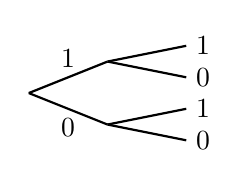
\begin{tikzpicture}
    	            \draw[thick] (0,0)--(1,0.4);
    	            \draw[thick] (0,0)--(1,-0.4);
    	            
    	            \draw (0.5,0.2) node[anchor=south] {$1$};
    	            \draw (0.5,-0.2) node[anchor=north] {$0$};
    	            
    	            \draw[thick] (1,0.4)--(2,0.6);
    	            \draw[thick] (1,0.4)--(2,0.2);
    	            \draw[thick] (1,-0.4)--(2,-0.2);
    	            \draw[thick] (1,-0.4)--(2,-0.6);
    	            
    	            \draw (2,0.6) node[anchor=west] {$1$};
    	            \draw (2,0.2) node[anchor=west] {$0$};
    	            \draw (2,-0.2) node[anchor=west] {$1$};
    	            \draw (2,-0.6) node[anchor=west] {$0$};
    	        \end{tikzpicture}
	        \end{center}
	        Since there are \( n \) elements, there are \( 2^n \) possible selections. Note that with a slight modification, this argument can be generalized to prove the multiplication principle. 
	        
	        \item For each \( 0 \leq k \leq n \), there are \( {n \choose k} \) \(k\)-element subsets of \( S \). Thus, using the Binomial Theorem 
	        \[ \sum_{k=0}^n {n \choose k} = \sum_{k=1}^n {n \choose k} (1)^{n-k} (1)^k = (1+1)^n = 2^n \]
	    \end{enumerate}
	\end{proof}
\end{exercise}

\begin{exercise} \label{0.102}
	pending
\end{exercise}

\begin{exercise} \label{0.103}
	pending
\end{exercise}

\begin{exercise} \label{0.104}
	pending
\end{exercise}

\begin{exercise} \label{0.105}
	pending
\end{exercise}

\begin{exercise} \label{0.106}
	pending
\end{exercise}

\begin{exercise} \label{0.107}
	pending
\end{exercise}

\begin{exercise} \label{0.108}
	pending
\end{exercise}

\begin{exercise} \label{0.109}
	pending
\end{exercise}

\begin{exercise} \label{0.110}
	pending
\end{exercise}

\begin{exercise} \label{0.111}
	pending
\end{exercise}

\begin{exercise} \label{0.112}
	pending
\end{exercise}

\begin{exercise} \label{0.113}
	pending
\end{exercise}

\begin{exercise} \label{0.114}
	pending
\end{exercise}

\begin{exercise} \label{0.115}
	pending
\end{exercise}

\begin{exercise} \label{0.116}
	pending
\end{exercise}


